%%%%%%%%%%%%%%%%%%%%%%%%%%%%%%%%%%%%%%%%%%%%%%%%%%%%%%%%%%%%%%%%%%%%%%%%%%%%%%%%
%% 서울대학교 데이터마이닝연구실 구성원들의 박사학위논문 작성을 위해 아래 저작자의 자료를 일부 수정하였습니다.
%% Author: zeta709 (zeta709@gmail.com) 
%%%%%%%%%%%%%%%%%%%%%%%%%%%%%%%%%%%%%%%%%%%%%%%%%%%%%%%%%%%%%%%%%%%%%%%%%%%%%%%%
%% 2016-12-23 한글 석사 논문을 위해 추가 수정 by 양호성 hoseong@dm.snu.ac.kr
%% 2018-01-08 산업공학과 데이터마이닝 전공을 산업공학과로 수정하고, 편리한 작업을 위한 추가 수정 및 팁 작성 by 문지형 jhmoon@dm.snu.ac.kr

\RequirePackage{fix-cm} 
% oneside : 단면 인쇄용
% twoside : 양면 인쇄용
% phd/ms : 박사 / 석사
% openright : 챕터가 홀수쪽에서 시작
% ko : 한글 논문
\documentclass[ko,indentfirst,twoside,ms]{snuthesis_utf8}

%%%%%%%%%%%%%%%%%%%%%%%%%%%%%%%%%%%%%%%%
%% 목차 양식을 변경하는 코드
%% subfigure (subfig) package 사용 여부에 따라
%% tocloft의 옵션을 다르게 지정해야 한다.
%\usepackage[titles,subfigure]{tocloft} % when you use subfigure package
\usepackage[titles]{tocloft} % when you don't use subfigure package
\makeatletter % don't delete me
\renewcommand\cftchappresnum{Chapter~}
\renewcommand\listfigurename{그림~목차}
\renewcommand\listtablename{표~목차}
\renewcommand\cftfigpresnum{그림~}
\renewcommand\cfttabpresnum{표~}
\renewcommand\figurename{그림~}
\renewcommand\tablename{표~}
\renewcommand\bibname{참고문헌}
\renewcommand\contentsname{목~~~차}
\renewcommand\cftchapafterpnum{\vskip2pt}
\renewcommand\cftsecafterpnum{\vskip2pt}
% \renewcommand\listoftables{표~목차}

\usepackage[pdftex,bookmarks=true]{hyperref}
\usepackage{tabularx}
\usepackage{array,multirow,graphicx,rotating,booktabs}
\usepackage{caption}  %subfigure
\usepackage{subcaption}  %subfigure
\usepackage[round, sort, numbers]{natbib} %reference style
\newcommand\mycite[1]{[\citenum{#1}]}
\newcommand\myauthor[1]{\citeauthor{#1} (\citeyear{#1})}
\usepackage{pbox} % line break in table
\usepackage{adjustbox}
\usepackage{footnote}
\usepackage{color}
\usepackage{colortbl}
\usepackage{amsmath}
\usepackage{float} % position here
\usepackage{lscape} % for landscape page
\usepackage{kotex}
%\usepackage[driverfallback=dvipdfm]{hyperref}


\makeatother % don't delete me
\newlength{\mytmplen}
\settowidth{\mytmplen}{\bfseries\cftchappresnum\cftchapaftersnum}
\addtolength{\cftchapnumwidth}{\mytmplen}
\settowidth{\mytmplen}{\bfseries\cftfigpresnum\cftfigaftersnum}
\addtolength{\cftfignumwidth}{\mytmplen}
\settowidth{\mytmplen}{\bfseries\cfttabpresnum\cfttabaftersnum}
\addtolength{\cfttabnumwidth}{\mytmplen}
%% 목차 양식을 변경하는 코드 끝
%%%%%%%%%%%%%%%%%%%%%%%%%%%%%%%%%%%%%%%%

%%%%%%%%%%%%%%%%%%%%%%%%%%%%%%%%%%%%%%%%
%% 다른 패키지 로드
%% http://faq.ktug.or.kr/faq/pdflatex%B0%FAlatex%B5%BF%BD%C3%BB%E7%BF%EB
%% 필요에 따라 직접 수정 필요
\ifpdf
	% \input glyphtounicode\pdfgentounicode=1 %type 1 font사용시
	%\usepackage[pdftex,unicode]{hyperref} % delete me
	%\usepackage[pdftex]{graphicx}
	%\usepackage[pdftex,svgnames]{xcolor}
\else
	%\usepackage[dvipdfmx,unicode]{hyperref} %로 delete me%
	%\usepackage[dvipdfmx]{graphicx}
	%\usepackage[dvipdfmx,svgnames]{xcolor}
\fi
%%%%%%%%%%%%%%%%%%%%%%%%%%%%%%%%%%%%%%%%
%
%% \title : 22pt로 나오는 큰 제목
%% \title* : 16pt로 나오는 작은 제목
\title{한글논문제목입니다 \\ 너무길면 밑으로}
\title*{Korean title to English}

\titlen{Korean title to English}

\author{홍길동}
\author*{홍길동} % Same as \author.
\authorn{홍~길~동}
\phonenumber{010-1111-1111}
\studentnumber{2016-11111}
\advisor{Nada~Ga}
\advisor*{조성준}
\advisorn{조 성 준}
\graddate{2018~년~~2~월}
\submissiondate{2018~년~~2~월}
\submissiondaten{2018~년~~2~월~~1~일}
\approvaldate{2017~년~~12~월}

\committeemembers%
{교 수 님}%
{조 성 준}%
{교 수 님}%
{교 수 님}%
{교 수 님} %

%% Length of underline
\setlength{\committeenameunderlinelength}{5cm}

 
\begin{document}
\pagenumbering{Roman}
\makefrontcover
\makeapproval

%agreement page
% \cleardoublepage
% \makeagreement

\clearpage
\pagenumbering{roman}

\keywordalt{키워드 1, 키워드 2}

\begin{abstractalt}
초록...
\end{abstractalt}
\clearpage

% % 여기 수정할 것

\addcontentsline{toc}{chapter}{\contentsname}
\tableofcontents
\clearpage

\addcontentsline{toc}{chapter}{\listtablename}
\listoftables
\clearpage

\addcontentsline{toc}{chapter}{\listfigurename}
\listoffigures
\clearpage

\pagenumbering{arabic}

\chapter{서론}
이 가이드는 졸업논문 latex template에 생소한 졸업 예정자들을 위해 (빠른 문서작업을 위해) 만들어졌다.
평소에 쓰던 latex 문법에 약간의 꿀팁만을 첨가하여 조금 더 편리하게 사용할 수 있도록 도움을 주고자 한다.


\chapter{관련 꿀팁}
\section{이미지 삽입}
이미지 삽입을 위해 'figure'라는 폴더를 만들어두는 것이 편하다.
일단 tex file이 compile되면 지저분한 파일이 많이 생기는데, 여기에 더해 이미지 파일까지 같은 경로에 있으면 머리가 아프다.


\begin{figure}[h]
	\centering
	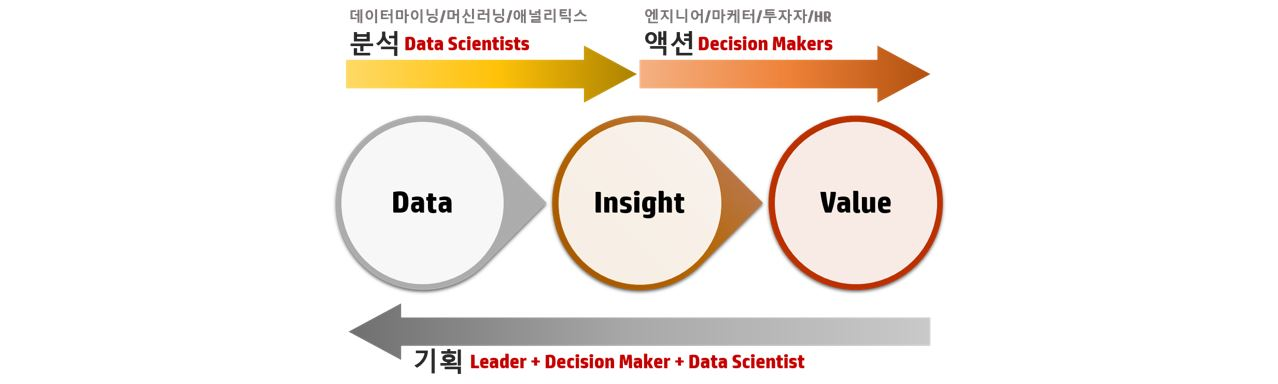
\includegraphics[width=1\textwidth]{figure/div.png}  % scale보다는 문서크기를 보고 width의 비율로 정하는 편이 크기 조정할 때 직관적이다. 예시 그림의 경우에는 원래 가로 여백이 있었다.
	\caption{Data, Insight, Value}
	\label{fig:div}
\end{figure}


\clearpage 
\section{표 삽입}
\subsection{기본}
\url{https://www.tablesgenerator.com/latex_tables} 에서 가장 기본적인 template을 만들어준다!

\clearpage
\subsection{응용}
latex 작업에서 제일 짜증나는 부분은 표 삽입이다.
크기 조절, highlight, 주석달기 등이 한글에 비해 굉장히 귀찮아서 많은 사람들이 표 때문에 hwp로 돌아서는 경우가 있다.
하지만 졸업논문 작성을 위해 다음에서 소개하는 것만 익히면 latex이 훨씬 편하게 느껴질 것이다.

\textit{adjustbox}: 표의 전체 크기를 조절하는 장치다. 없는 경우, 문서 범위를 넘어가는 표가 생성될 수 있다.

\textit{columncolor}: 내 모델의 결과를 강조하기 위해 column전체에 음영을 넣을 수 있는 장치다.

\textit{footnotemark와 footnotetext}: 표 내부에서는 footnote가 명령어가 먹히지 않는다. 이 때, footnotemark와 footnotetext를 사용하면 주석을 달 수 있다.
주의해야 할 점은, 주석이 달리는 페이지가 항상 표와 같지 않다는 (...) 것인데, 잘 맞춰보자.
그리고 footnotemark가 표 내부에 여러 번 달리면 주석 번호가 이상해지는데, 이 때를 위해 \textit{addtocounter}가 있으니 예시를 보고 잘 사용해보자.
\newline
\newline
이 이상으로 필요한 경우에는 열심히 구글링을 하자.

\clearpage
\begin{table}[h]
\centering
	\caption{Average error rate on bAbI story-based tasks with 10k training samples}
	\label{table:babi_result}
\begin{adjustbox}{max width=0.95\textwidth}
\begin{tabular}{l|llllllll>{\columncolor[gray]{0.8}}l}
\hline
Task                                 & \multicolumn{1}{c}{MemNN} & \multicolumn{1}{c}{MemN2N} & \multicolumn{1}{c}{GMemN2N} & \multicolumn{1}{c}{DMN} & \multicolumn{1}{c}{DMN+} & \multicolumn{1}{c}{DNC} & \multicolumn{1}{c}{EntNet\footnotemark}& \multicolumn{1}{c}{RN\footnotemark} & \multicolumn{1}{c}{RMN} \\ \hline
1: Single Supporting Fact            & \textbf{0.0}                       & \textbf{0.0}                        & \textbf{0.0} & \textbf{0.0}                     & \textbf{0.0}                      & \textbf{0.0}                     & \textbf{0.1}                        & \textbf{0.0}                    & \textbf{0.0}                     \\
2: Two Supporting Facts              & \textbf{0.0}                       & \textbf{0.3}                        & \textbf{0.0}                         & \textbf{1.8}                     & \textbf{0.3}                      & \textbf{0.4}                     & \textbf{2.8} & 8.3                    & \textbf{0.5}                     \\
3: Three Supporting Facts            & \textbf{0.0}                       & 9.3                        & \textbf{4.5                        } & \textbf{4.8}                     & \textbf{1.1}                      & \textbf{1.8}                     & 10.6                       & 17.1                  & 14.7                     \\
4: Two Argument Relations            & \textbf{0.0}                       & \textbf{0.0}                        & \textbf{0.0} & \textbf{0.0}                     & \textbf{0.0}                    & \textbf{0.0}                    & \textbf{0.0} & \textbf{0.0}                    & \textbf{0.0}                   \\
5: Three Argument Relations          & \textbf{2.0 }                      & \textbf{0.6}                        & \textbf{0.2 } & \textbf{0.7}                     & \textbf{0.5}                     &\textbf{0.8}                     &\textbf{0.4}                       & \textbf{0.7}                   & \textbf{0.4}                     \\
6: Yes/No Questions                  & \textbf{0.0}                       & \textbf{0.0}                        & \textbf{0.0} & \textbf{0.0}                     & \textbf{0.0}                      & \textbf{0.0}                     & \textbf{0.3}                       & \textbf{0.0}                    & \textbf{0.0}                     \\
7: Counting                          & 15.0                      & \textbf{3.7}                       & \textbf{1.8}                         & \textbf{3.1}                     & \textbf{2.4}                      & \textbf{0.6}                    & \textbf{0.8}                        &\textbf{0.4}                &\textbf{0.5}                    \\
8: Lists/Sets                        & 9.0                       & \textbf{0.8}                        & \textbf{0.3}                         & \textbf{3.5}                     & \textbf{0.0}                     & \textbf{0.3}                     &\textbf{0.1} & \textbf{0.3}                   & \textbf{0.3}                     \\
9: Simple Negation                   & \textbf{0.0}                       & \textbf{0.8}                        & \textbf{0.0}                         & \textbf{0.0 } & \textbf{0.0}                      & \textbf{0.2}                     &\textbf{ 0.0 }                       & \textbf{0.0}                   &\textbf{0.0}                    \\
10: Indefinite Knowledge             & \textbf{2.0}                       & \textbf{2.4}                      & \textbf{0.2} &\textbf{2.5}                     & \textbf{0.0}                      & \textbf{0.2}                     & \textbf{0.0}                        & \textbf{0.0}                    & \textbf{0.0}                   \\
11: Basic Coreference                & \textbf{0.0}                       & \textbf{0.0}                        & \textbf{0.0}                         & \textbf{0.1}                    & \textbf{0.0}                      & \textbf{0.0}                     & \textbf{0.0}                        & \textbf{0.4}                  & \textbf{0.5}                    \\
12: Conjunction                      & \textbf{0.0}                       & \textbf{0.0}                        & \textbf{0.0}                         & \textbf{0.0}                     &\textbf{0.0}                      &\textbf{0.0}                     & \textbf{0.0}                        & \textbf{0.0}                   & \textbf{0.0}                     \\
13: Compound Coreference             & \textbf{0.0}                       & \textbf{0.0}                        & \textbf{0.0} & \textbf{0.2}                     & \textbf{0.0}                      & \textbf{0.1} & \textbf{0.0}                        & \textbf{0.0}                 & \textbf{0.0}                     \\
14: Time Reasoning                   & \textbf{1.0}                       &\textbf{0.0}                        & \textbf{0.0}                         &\textbf {0.0}                     & \textbf{0.0}                      & \textbf{0.4} & \textbf{3.6}                      &\textbf{0.0}                    & \textbf{0.0}                    \\
15: Basic Deduction                  & \textbf{0.0}                       & \textbf{0.0}                        &\textbf{0.0}                         & \textbf{0.0}                    &\textbf{0.0}                    & \textbf{0.0}                     &\textbf{0.0}                        & \textbf{0.0}                   &\textbf{0.0}                     \\
16: Basic Induction                  &\textbf{0.0}                       & \textbf{0.4}                        & \textbf{0.0}                         & \textbf{0.6}                   & 45.3                     & 33.1                    & 52.1                       & \textbf{4.9}                   & \textbf{0.9}                    \\
17: Positional Reasoning             & 35.0                        & 40.7                       & 27.8                        & 40.4                    & \textbf{4.2}                      & 12.0                    & 11.7                       & \textbf{1.6}                    & \textbf{0.3} \\
18: Size Reasoning                   & \textbf{5.0}                      & 6.7                        & 8.5                         & \textbf{4.7}                     & \textbf{2.1}                     & \textbf{0.8}                     & \textbf{2.1}                        & \textbf{2.1}                    & \textbf{2.3}                     \\
19: Path Finding                     & 64.0                      & 66.5                       & 31.0                        & 65.5                    & \textbf{0.0}                      & \textbf{3.9}                     & 63.0                       & \textbf{3.2}                    & \textbf{2.9}                     \\
20: Agent's Motivations              & \textbf{0.0}                       & \textbf{0.0}                        & \textbf{0.0} & \textbf{0.0}                    &\textbf{ 0.0}                      & \textbf{0.0}                     & \textbf{0.0}                        &\textbf{0.0}                    & \textbf{0.0}                     \\ \hline
Mean error (\%)                      & 6.7                       & 6.6                        & 3.7                         & 6.4                     & 2.8                      & 2.7                     & 7.4                        & 2.0                    & \textbf{1.2}                     \\
Failed tasks (err. \textgreater  5\%) & 4                         & 4                          & 3                           & 2                       & \textbf{1}                        & 2                       & 4                          & 2                       & \textbf{1}                       \\ \hline
\end{tabular}
\end{adjustbox}
\end{table}

\addtocounter{footnote}{-1}
\footnotetext{For a fair comparison, we report EntNet's result~\mycite{henaff2016tracking} which was jointly trained on all tasks. It was written in the appendix of the paper.}
\addtocounter{footnote}{+1}
\footnotetext{Our implementation. The result is different from what \myauthor{santoro2017simple} mentioned, which is caused by the initialization~\mycite{santoro2017simple}.}

\chapter{참고문헌 넣기}
\section{마침표 직전에 넣는 경우}
참고문헌을 넣기 위해 기존의 $\sim\setminus$cite\{\} 를 사용하면 안된다. 

예시: ... 라고 말했다~\cite{bishop2006}.
\newline

( ) 부분 때문인데, 이를 [ ]로 바꾸고자 위에서 mycite를 따로 정의해주었다.

예시: ... 라고 말했다~\mycite{bishop2006}.

\clearpage
\section{저자 이름으로 넣는 경우}

reference를 저자 명으로 넣어야 할 때가 있다. 이를 위해 위에서 myauthor를 따로 정의해주었다.

예시: \myauthor{bishop2006} 는 ... 라고 말했다~\mycite{bishop2006}.


\begin{bibpage}
	\bibliographystyle{plainnat}
	\bibliography{ref}
\end{bibpage}

\appendix
\chapter{부록제목 1}
부록은 table of contents에 제대로 뜨지 않는다.
이 때는 .toc 파일을 열어서 (혹은 table of contents에서 ctrl을 누른 상태로 클릭해보자) Bibliography 밑에 한줄을 추가해주면 아래처럼 된다.

\contentsline {chapter}{Bibliography}{11}{section*.9} % 현재 Bibliography
\contentsline {chapter}{Appendix}{12}{section*.10} % {12}는 페이지 번호이므로 알아서 맞추자
\contentsline {section}{\numberline {A}부록제목 1}{12}{section.Alph0.1}
\contentsline {section}{\numberline {B}부록제목 2}{13}{section.Alph0.2}


\chapter{부록제목 2}


\keyword{Keyword 1, Keyword 2}
\begin{abstract}
English version abstract
\end{abstract}
\end{document}

